\documentclass{article}
\usepackage[utf8]{inputenc}
\usepackage{hyperref}



\title{Les Réseaux de Neurones Convolutionnels (RNC)}

\date{June 2021}

\usepackage{natbib}
\usepackage{graphicx}
\usepackage{graphicx}
\usepackage{fullpage}
\usepackage{eso-pic}
\usepackage{listings}
\usepackage{ulem}
\usepackage{float}
\usepackage{comment}


\begin{document}

\maketitle



Durée : 25 mn

\section{Prérequis}

\begin{itemize}
\item Notions de programmation et d'algorithmique primaires
\item Capsule \textit{Généralités réseaux de neurones et deep-learning}
\end{itemize}


\section{Acquis d'apprentissage}

\begin{itemize}
\item Introduction aux réseaux de neurones convolutionnels
\end{itemize}


\section{Principes généraux}


En deep-learning, les Réseaux de Neurones Convolutionnels (RNC, en anglais \textit{CNN : Convolutionnal Neural Network}) 
proposent des structures particulièrement efficaces pour l'analyse du contenu des images. 
\\
Pour cela les RNC mettent en oeuvre des traitements et une architecture et bien spécifiques :
\begin{itemize}
\item l'extraction des caractéristiques des images (\textit{features}) à l'aide de filtres convolutifs,
\item la réduction de la quantité d'information générée par la convolution avec des filtres de \textit{pooling},
\item une architecture qui empile des couches "convolution $\rightarrow$ activation $\rightarrow$ pooling..." chargées d'extraire les caractéristiques
de l'image, qui sont au final applaties et envoyées en entrée d'un réseau dense séquentiel 
chargé de l'étape ultime de classification.
\end{itemize}

\begin{figure}[H]
\centering
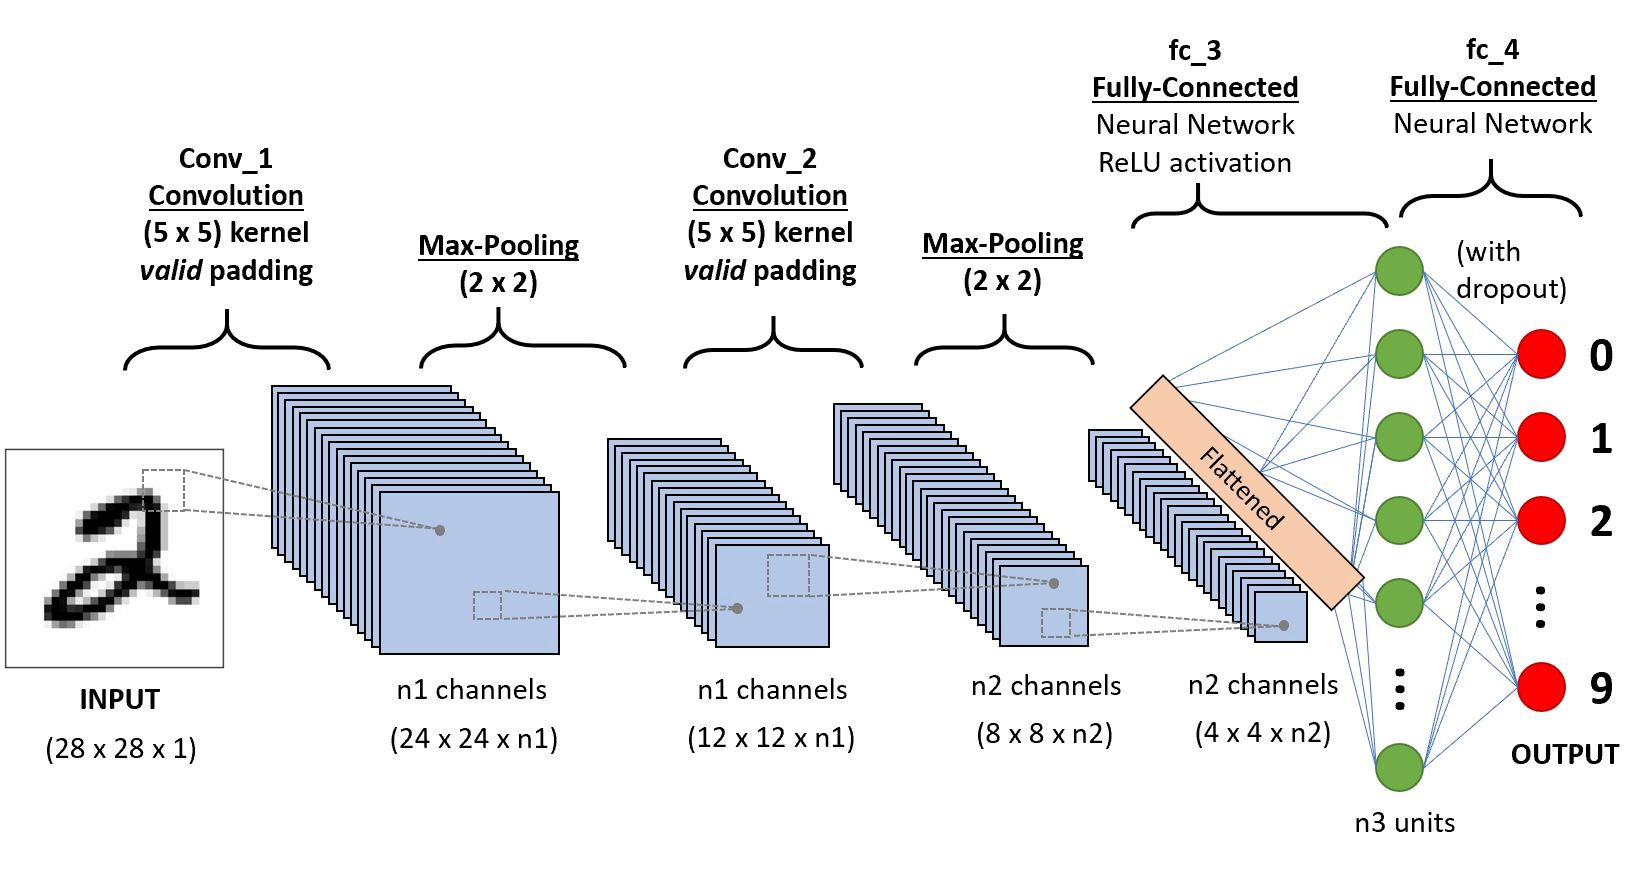
\includegraphics[width=1\textwidth]{img/cnn.jpeg}
\medskip
[https://www.analyticsvidhya.com/blog/2020/10/what-is-the-convolutional-neural-network-architecture/]
\end{figure}


On peut noter qu'un RNC effectue des traitements sur l'image en entrée 
avant de basculer sur un réseau de neurone dense comme vu précédement.
Un exemple de structure d'un RNC inspiré du réseau \textbf{LeNet5}
est affiché dans la figure ci-dessous. 
C'est un des premiers RNC proposé par Yann LeCun *et al.* 
dans les années 90 pour la reconnaisannce des images MNIST :

\begin{figure}[H]
\centering
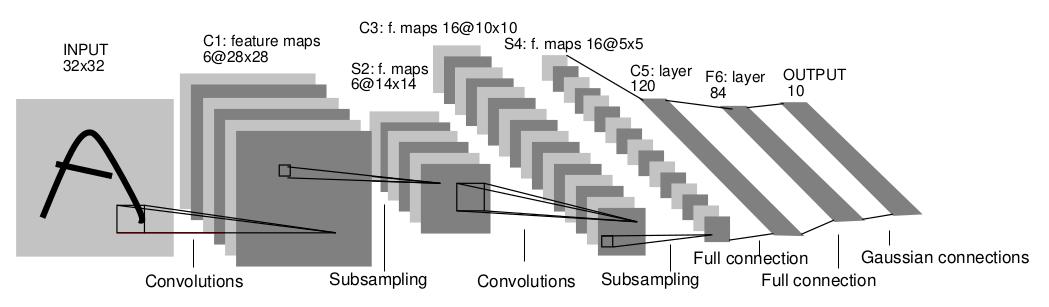
\includegraphics[width=1\textwidth]{img/LeNet5.png}
\medskip
[Lecun, Y.; Bottou, L.; Bengio, Y.; Haffner, P. (1998). "Gradient-based learning applied 
to document recognition". Proceedings of the IEEE. 86 (11): 2278–2324. doi:10.1109/5.726791.]
\end{figure}

\newpage

\section{Extraction des caractéristiques d'une image avec un filtre de convolution}



\begin{figure}[H]
\begin{minipage}[c]{0.4\linewidth}

On rappelle que la représentation informatique d'une image RGB (Red, Green, Blue) 
repose sur 3 matrice de pixels (une pour chaque couleur) constituant un tableau à 
3 dimensions (witdh, heihgt, color).

Une image en ton de gris ne nécessite qu'une seule matrice. 
Dans un soucis de simplification, la suite présente le cas des images en ton de gris.

\end{minipage} \hfill
\begin{minipage}[c]{0.6\linewidth}

\begin{figure}[H]
\centering
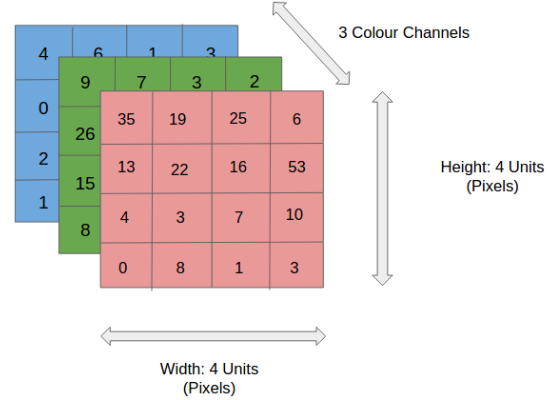
\includegraphics[width=0.8\textwidth]{img/rgb.png}
\medskip
[https://towardsdatascience.com/a-comprehensive-guide-to-convolutional-neural-networks-the-eli5-way-3bd2b1164a53]
\end{figure}


\end{minipage}
\end{figure}


\begin{figure}[H]
\begin{minipage}[c]{0.4\linewidth}

La convolution d'une image par un filtre (aussi appelé noyau, \textbf{kernel}) revient à déplacer
une \textit{petite fenêtre 2D} ( 3x3, 5x5 ....) sur l'image et à calculer à chaque fois le produit 
tensoriel contracté entre les élements du filtre et les pixels de l'image délimités par 
le filtre (somme des produits terme à terme).

\end{minipage} \hfill
\begin{minipage}[c]{0.6\linewidth}

\begin{figure}[H]
\centering
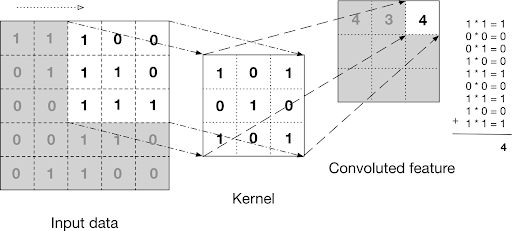
\includegraphics[width=0.9\textwidth]{img/grayscale.png}
\medskip
[http://www.davidsbatista.net/blog/2018/03/31/ \\
SentenceClassificationConvNets/]
\end{figure}


\end{minipage}
\end{figure}

L'animation ci-dessous illustre la convolution d'une image 5x5 par un filtre 3x3 sans \textit{padding} 
sur les bords : on obtient une nouvelle image plus petite de 3x3 pixels.

\newpage

\begin{figure}[H]

\begin{figure}[H]
\minipage{0.32\textwidth}
  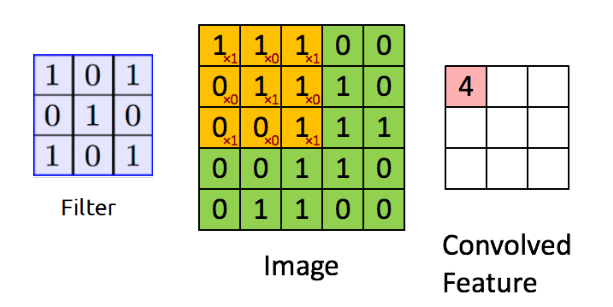
\includegraphics[width=\linewidth]{img/conv1.png}
\endminipage\hfill
\minipage{0.32\textwidth}
  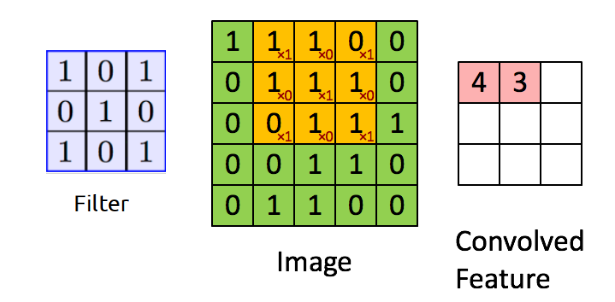
\includegraphics[width=\linewidth]{img/conv2.png}
\endminipage\hfill
\minipage{0.32\textwidth}%
  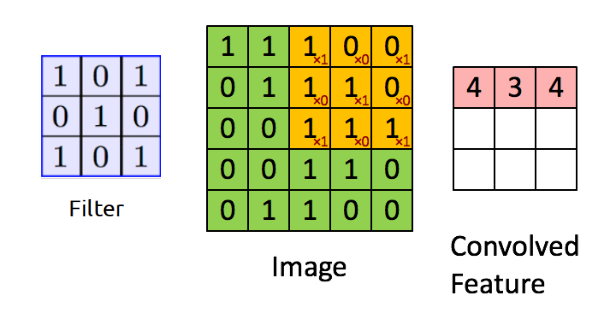
\includegraphics[width=\linewidth]{img/conv3.png}
\endminipage
\end{figure}

\begin{figure}[H]
\minipage{0.32\textwidth}
  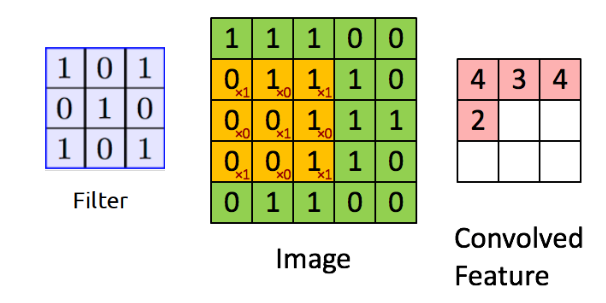
\includegraphics[width=\linewidth]{img/conv4.png}
\endminipage\hfill
\minipage{0.32\textwidth}
  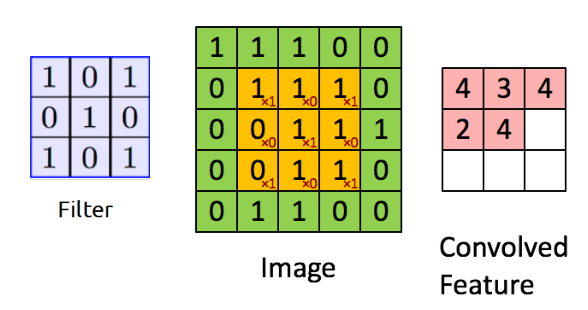
\includegraphics[width=\linewidth]{img/conv5.png}
\endminipage\hfill
\minipage{0.32\textwidth}%
  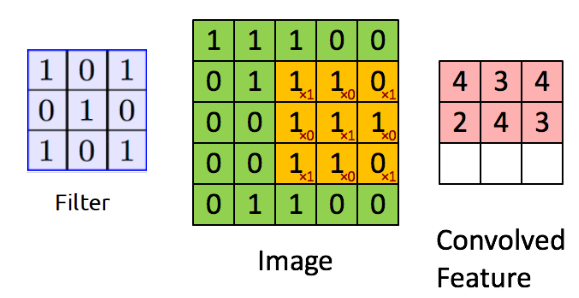
\includegraphics[width=\linewidth]{img/conv6.png}
\endminipage
\end{figure}

\begin{figure}[H]
\minipage{0.32\textwidth}
  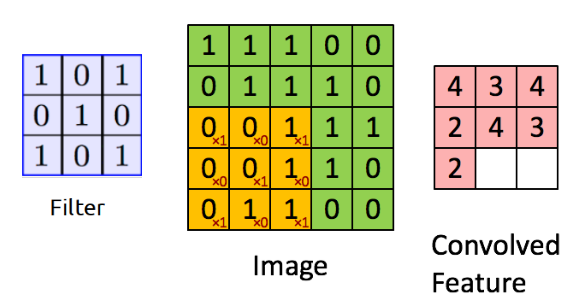
\includegraphics[width=\linewidth]{img/conv7.png}
\endminipage\hfill
\minipage{0.32\textwidth}
  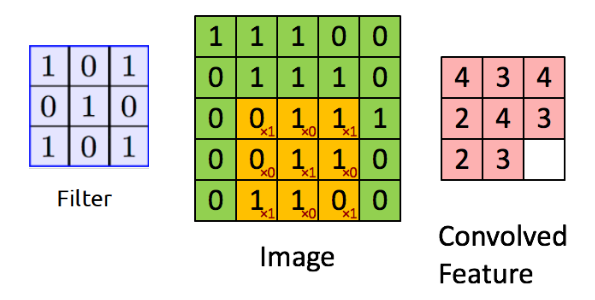
\includegraphics[width=\linewidth]{img/conv8.png}
\endminipage\hfill
\minipage{0.32\textwidth}%
  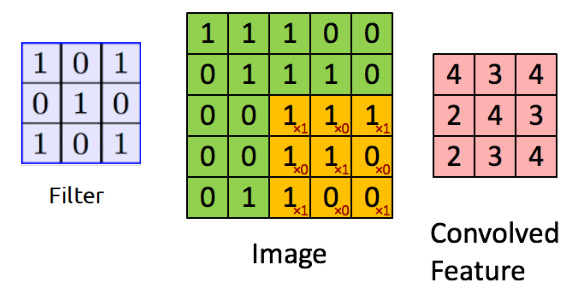
\includegraphics[width=\linewidth]{img/conv9.png}
\endminipage
\end{figure}

\medskip
[http://deeplearning.stanford.edu/tutorial]
\end{figure}

Pour conserver la taille de l'image d'entrée, on peut faire appel à une technique 
de \textit{padding} pour créer de nouvelles données sur les bords de l'image (par dupplication 
des données sur les bords, ou ajout de lignes et colonnes de 0... par exemple) : 


\begin{figure}[H]
\begin{minipage}[c]{0.4\linewidth}

Le but de la convolution est d'extraire des caractéristiques particulières présentes
dans l'image source : on parle de "carte des caratéristiques" (\textit{feature map}) 
pour désigner l'image produite par l'opération de convolution. 
L'état de l'art conduit à utiliser plusieurs filtres convolutifs 
pour extraire des caractéristiques différentes : on peut avoir jusqu'à 
plusieurs dizaines de filtres convolutifs dans un même couche du réseau 
qui génèrent autant de \textit{feature map}, d'où l'augmentation des données crées
par ces opérations de convolution...

\end{minipage} \hfill
\begin{minipage}[c]{0.6\linewidth}

\begin{figure}[H]
\centering
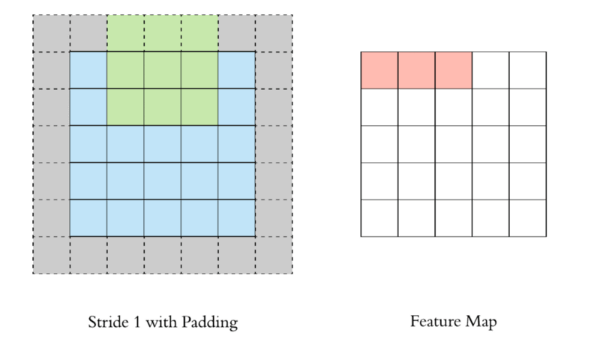
\includegraphics[width=1\textwidth]{img/conv.png}
\medskip
[https://towardsdatascience.com/applied-deep-learning-part-4-convolutional-neural-networks-584bc134c1e2"]
\end{figure}

\end{minipage}
\end{figure}


\subsection{Exemples d'extraction de caractéristiques avec des filtres convolutifs 
connus (\href{https://fr.wikipedia.org/wiki/Filtre_de_Prewitt}{filtre de Prewitt}):}

À titre d'exemple, la figure ci-dessous montre les \textit{features maps} obtenues en 
convoluant une image MNIST (un chiffre 7) avec 4 filtres 3x3 connus en traitement d'image
(filtres de Prewitt pour l'extraction de contours):

\begin{figure}[H]
\centering
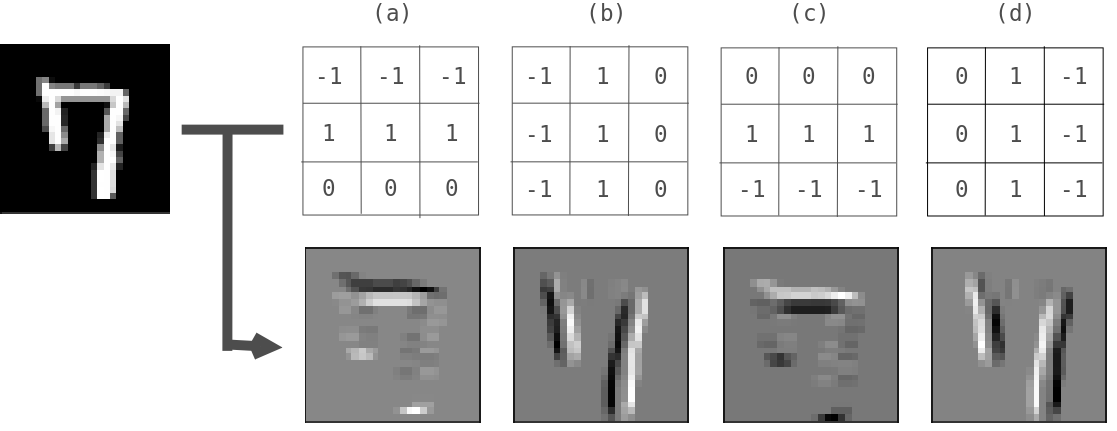
\includegraphics[width=0.8\textwidth]{img/7_mnist_4_filtres.png}
\medskip
[crédit image : JLC]
\end{figure}

On voit que ces filtres agissent comme des filtres de détection de contour : 
dans les images de sortie, les pixels les plus blancs constituent ce que les filtres ont détecté :

\begin{itemize}
\item les filtre (a) et (c) détectent des contours horizontaux inférieurs et supérieurs,
\item les filtre (b) et (d) détectent des contours verticaux droite et gauche.
\end{itemize}

Ces exemples très simples permettent de comprendre comment fonctionne l'extraction des
\textit{features} d'une image par filtrage convolutif.

Il est important de comprendre que c'est l'apprentissage qui va trouver 
les valeurs des filtres de convolutionsqui conviennent le mieux à 
l'extraction des caractéristiques pertinentes du jeu d'images fournies.

\subsection{Cas général : images RGB traitée par plusieurs filtres de convolution}


Dans le cas général des images couleurs (RGB), le filtre de convolution est composé des 3 matrices. 
L'opération reste identique : pour une position du filtre de convolution sur l'image, 
le produit tensoriel contracté du filtre avec le sous-tableau 3D correspondant 
dans l'image fournit un nombre scalaire, et le balayage du procédé sur toute l'image 
donne la matrice des caractéristiques (\textit{feature map}) de l'image. 

Par exemple si l'on utilise 10 filtres de convolution RGB 5x5 (10 tableaux de dimensions (5,5,3)) 
pour traiter (avec  \textit{padding}) une image RGB de 32x32 pixels 
(tableau de dimensions (32,32,3), on obtient une \textit{feature maps} de dimensions (32,32,10), 
soit 10240 termes alors que l'image source n'en a que 1024 !


\begin{figure}[H]
\begin{minipage}[c]{0.4\linewidth}


\begin{figure}[H]
\centering
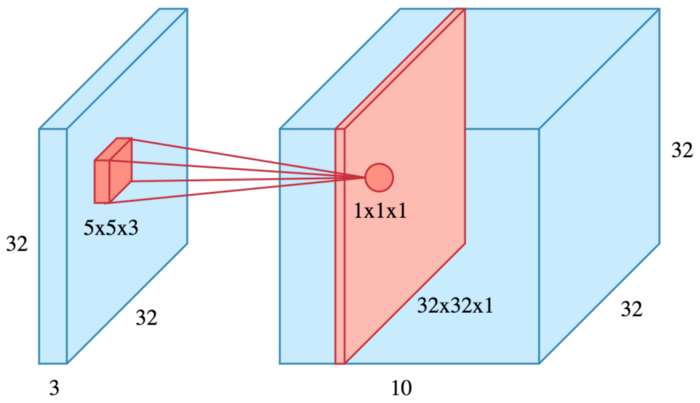
\includegraphics[width=1\textwidth]{img/conv_3D_10.png}

\medskip
[https://towardsdatascience.com/applied-deep-learning-part-4-convolutional-neural-networks-584bc134c1e2]

\end{figure}
\end{minipage} \hfill
\begin{minipage}[c]{0.6\linewidth}

\begin{figure}[H]
\centering
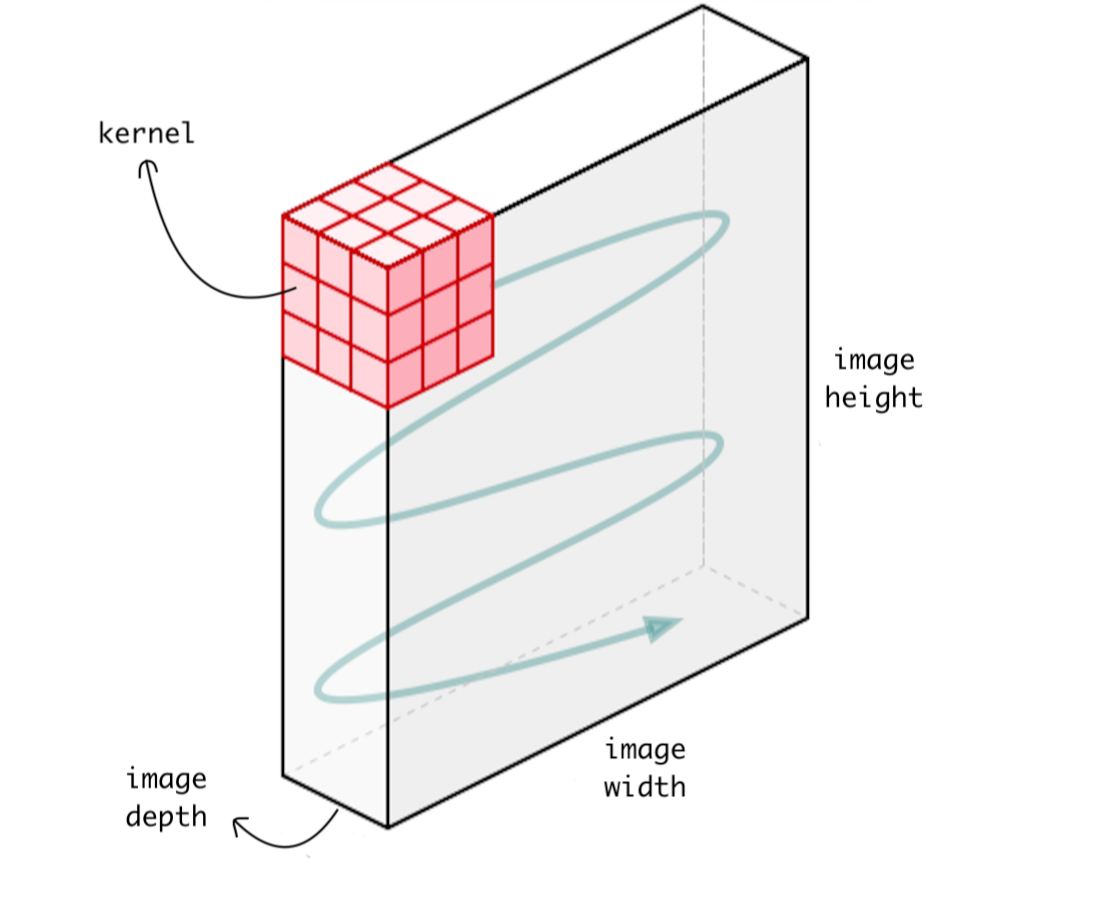
\includegraphics[width=0.8\textwidth]{img/schemaRGB.png}

\medskip
[https://towardsdatascience.com/understanding-1d-and-3d-convolution-neural-network-keras-9d8f76e29610]
   
\end{figure}

\end{minipage}
\end{figure}


Pour réduire la quantité d'information générée par les filtres 
de convolution sans perdre trop d'information, 
la convolution est toujours suivie d'une opération de \textit{pooling}.

\subsection{Du filtre convolutif à la couche de neurones convolutifs}

L'intégration du filtrage convolutif dans la structure du réseau de neurones donne l'organisation des calculs  suivante :

\begin{itemize}
\item Chaque filtre convolutif posssède les mêmes coefficients pour les 3 couleurs : 
pour le réseau LeNet5 par exemple, chacun des 6 filtres 5x5x3 de la première couche 
possède seulement 25 coefficients, identiques pour les couleurs R, G, B.
\item Chaque unité (neurone convolutif) d'une \textit{feature map} de la couche C1 reçoit 75 pixels
(25 pixels rouges $R_i$, 25 pixels vert $G_i$ et 25 pixels bleus $B_i$) 
délimités par la position du filtre convolutif dans l'image source.
\item Le neurone $k$ d'une \textit{feature map} calcule une sortie 
$y_k = F_a(\sum_{i=1}^{25}{\omega_i(R_i + G_i + B_i) - b_k})$, 
où $b_k$ est le biais du neurone $k$ et $F_a$ la fonction d'activation (très souvent `relu`).
\item pour les 6 filtres convolutrifs de la couche C1, on a donc  6 x (25 + 1) paramètres, 
soit 156 paramètres inconnues pour cette couche qui seront déterminé par entraînement du réseau.
\end{itemize}


Le même schéma est utilisé dans toutes les couches convolutionnelles.


\section{Le pooling}

Le \textit{pooling} vise à réduire quantité de données à traiter. 
Comme pour l'opération de convolution, on déplace un filtre 
sur les éléments du tableau \textit{feature map} et à chaque position 
du filtre sur le tableau, on calcule un nombre représentant tous 
les éléments sélectionnés dans le filtre (par exemple la valeur maximale, ou la moyenne....). 
Mais contrairement à la convolution, on déplace le filtre sans recouvrement.
Dans l'exemple simplifié ci-dessous, le filtre \textit{max spool} 
transforme la matrice 8x8 en une matrice 4x4 qui décrit 
"à peu près" la même information mais avec moins de données :

\begin{figure}[H]
\centering
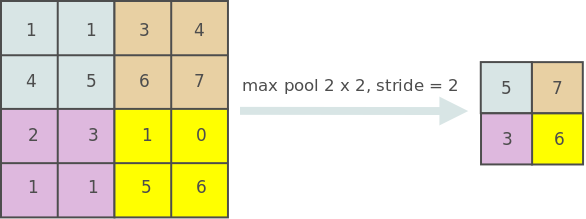
\includegraphics[width=0.7\textwidth]{img/max_pool_2x2.png}

\medskip

[crédit image : JLC]    
\end{figure}

\end{document}
